\section{Erfahrungen eines Analphabeten}


Nach einem Erfahrungsbericht eines Analphabeten, belegen sich viele der Tatsachen die im vorherigen Abschnitt \ref{sec:reasons} unter dem Punkt Bildung genannt wurden. Dabei geht es um Bernd Dahler, der zu der Zeit als er dieses Interview gab 36 war.\\


\begin{figure}[h]
	\centering
		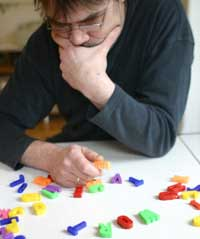
\includegraphics[scale=0.80]{Daten/BerndDahler.jpg}
	\caption{Bernd Dahler}
	\label{fig:BerndDahler}
\end{figure}



Hier hatte Bernd unter anderem geschildert, dass es weder f"ur ihn, noch f"ur seine Eltern leicht war. Er war das 2. j"ungste Kind in einer Familie mit 11 Kindern. In einer derart gro"sen Familie ist es wohl klar, wie die meisten sicher nachvollziehen k"onnen, dass die Kinder gr"o"stenteils sich selbst "uberlassen werden und auf die Bed"urfnisse der einzelnen Individuen nicht gro"s eingegangen werden kann, was bereits ein Grund daf"ur ist, dass Bernd in seiner Kindheit keine gro"se zus"atzliche Unterst"utzung aus der Familie bekam.\\

In der Schule hatte er bereits zum Anfang hin Probleme beim Lesen, weshalb er, wenn er laut vorlesen musste, stark stotterte, weshalb er stark ausgelacht wurde. Au"serdem wurde er von seinen Lehrern immerzu gen"otigt, dass er mit der rechten Hand schreiben solle, obwohl er Linksh"ander ist. Und wie man heutzutage von einigen Studien h"ort, soll dies der Entwicklung der Kinder nicht sonderlich gut tun.\\

Da Bernd den Anschluss nicht behielt und es nicht fertig brachte das Lesen im gleichen Tempo wie seine Mitsch"uler zu meistern, blieb er auf der Strecke. Daher spielte er meistens krank, wenn Klassenarbeiten geschrieben werden sollten. Den Lehrstoff an sich versuchte er mit schierer Aufmerksamkeit im Untericht aufzunehmen, was offensichtlich gereicht zu haben schien, um ihm einen Schulabschluss einzubringen. Selbstverst"andlich waren die Lehrer "uber seinen Zustand informiert und vermerkten seine Schw"ache auch in seinem Zeugnis.\\

 ALs er schlie"slich mit der Schule fertig war, versuchte er einen Job zu finden, in dem es keine starke Anforderungen an die Lese- bzw. Schreibf"ahigkeit gab. Somit kam er zu einer Ausbildung als Galvaniseur, welcher ein handwerklicher Beruf in dem zumeist mit Metallen gearbeitet wird. Diese Ausbildung dauerte f"ur ihn 3 Jahre und er durfte zum Ende hin seine Abschlusspr"ufung als reine m"undliche Pr"ufung absolvieren.\\

In seinem Privatleben gibt es niemanden unter seinen Freunden, der wei"s, dass er nicht lesen kann. Um dies unter anderen vor ihnen zu verbergen, bestellt er bspw. in Restaurants jedes mal Wienerschnitzel mit Pommes. Wenn er den Stadtplan lesen musste, hatte er einfach seine Brille vergessen und bat andere darum, ihm den Plan vorzulesen.\\

Sein Allgemeinwissen hat er auf einen guten Stand gebracht, indem er sich vieles was er im Fernsehen sieht einfach merkt, indem er Dokumentationen und "ahnliches schaut. Dumm ist Bernd nicht, nur hat er es leider in seiner Ausblidung aufgrund manglender Unterst"utzung nicht geschafft, das Lesen zu meistern.

